\subsubsection{Nuevos beneficios pagados en Jubilaciones y Pensiones}

\subsubsection{Nuevos beneficios pagados en Jubilaciones y Pensiones}

Como ya se describió en la sección anterior ``Prestaciones'', el IPS
otorga diferentes tipos de beneficios en función a los riesgos que se
cubren. En la Tabla xx se observa la evolución de la cantidad de los
nuevos beneficios pagados por tipo (de benefic io) desde el año xx al
2020. Se destaca un crecimiento considerable en la cantidad de nuevos
beneficios concedidos entre dichos años con una variación interanual
promedio en torno al xx\%.

En el Gráfico xx se ilustra la evolución de los nuevos beneficios
pagados (altas) en J y P por tipo, y se puede apreciar claramente que
hubo aumentos en la concesión de Jubilaciones Ordinarias, acompañado a
su vez de la implementación de la Jubilación P roporcional que en el
primer año tuvo un inicio importante para luego ir disminuyendo
gradualmente. La cantidad de nuevos beneficios pagados por Pensiones
Derechohabiente y Jubilaciones por Invalidez, se mantuvieron
prácticamente constantes a lo largo d el periodo considerado.

El aumento en el número de nuevos beneficios pagados se entiende que se
debe no solo a una evolución esperada en el incremento de beneficios,
sino también a una gran mejoría en las gestiones administrativas para la
concesión de los beneficios llegando a otorgar el beneficio al momento
de cumplir el requisito de edad (Plan Retiro Feliz).

Al mismo tiempo, se pone de manifiesto que el comportamiento de los
nuevos beneficios otorgados por Jubilación Proporcional se debe a que,
al existir nuevos requisitos para acogerse a la Jubilación, muchas
personas con aportes entre 15 y 25 años pudiero n acceder a un
beneficio, que de otra manera hubiera sido imposible.

En la Gráfica xx se observa la distribución porcentual (pesos relativos)
de los diferentes tipos de beneficios. En referencia a esto, desde el
año 2008 hasta el año 2010 se ha tenido una distribución similar, siendo
las Pensiones Derechohabiente y la J ubilación Ordinaria las de mayor
peso relativo, en torno al 35\% y al 60\% respectivamente. A partir del
año 2011 se evidencia una caída en la distribución de los porcentajes,
la cual se ha visto alterada por la inclusión de la Ley 4290/11 de la
Jubilac ión Proporcional.

Es normal que en los primeros años que se ha introducido una
modificación en las condiciones para acceder a los beneficios de la
etapa pasiva, se observe una gran demanda que luego irá disminuyendo
hasta estabilizarse.

Tanto en la Tabla xx y en el Gráfico xx se aprecia claramente como en el
transcurso de los 10 últimos años, los montos (nominales) pagados por
Jubilación Ordinaria han tenido una tendencia creciente, hasta llegar a
un promedio de Gs.xx. Del mismo modo, los montos de los beneficios
otorgados por Jubilación Proporcional y Pensiones Derechohabiente han
ido aumentando entre los años 2015 y 2020 llegando en promedio a Gs.xx y
Gs.xx respectivamente. En tanto que, los montos promedios de las
Jubilaciones p or Invalidez presentan un pico en el año 2016, para
sufrir un leve descenso en el año 2017, llegando a un promedio de
Gs.2.245.444 param dicho año. En cuanto al Complemento al SML, el mismo
posee un comportamiento prácticamente constante en el periodo c
onsiderado y su valor promedio ronda los Gs.200.000.

La Tabla xx y el Gráfico xx presentan la distribución porcentual de la
cantidad de nuevos pagos en J y P de enero a diciembre del año 2020. Con
respecto a las Jubilaciones por Invalidez hay una demanda desde los 20
años, especialmente importante entre l os 45 y 65 años. La Jubilación
Ordinaria, por su parte presenta alrededor del xx\% de los nuevos pagos
en los dos primeros tramos etarios, aproximadamente el xx\% corresponde
a la Jubilación Ordinaria Anticipada concedida entre los 55 y 59 años de
edad y xx\% para la Ordinaria concedida a partir de los 60 años de edad.
Los nuevos pagos otorgados en concepto de Jubilación Proporcional, están
concentrados en el tramo de edad que va de los 65 a 69 años, alcanzando
aproximadamente el xx\%. Por último, los pagos por PDH se encuentran
distribuidos a lo largo de todos los tramos etarios, presentando mayores
frecuencias en algunos tramos particulares como se puede apreciar en la
Tabla xx.

\textbf{***agregar la tabla de porcentaje de nuevos beneficios pagados en jubilación por invalidez, jubilación ordinaria, jubilación proporcional y pensión de derechohabiente, según tramo de edad***}

\textbf{***agregar el gráfico de distribución de la edad de retiro por tipo de prestación***}

\begin{table}[H]
\begin{center}
\caption{\bf{Evolución de la cantidad de nuevos beneficios pagados en Jubilaciones y Pensiones.}}
\begin{tabular}{l|rrrrrrrrrrrrrrr}
\scriptsize
%\begin{tabular}{llllllllll}
\cline{1-10}
\multicolumn{1}{c}{} &
  \multicolumn{9}{|c}{Año de inicio de pago del beneficio} \\
\multicolumn{1}{c}{} &
  \multicolumn{1}{|r}{2012} &
  \multicolumn{1}{r}{2013} &
  \multicolumn{1}{r}{2014} &
  \multicolumn{1}{r}{2015} &
  \multicolumn{1}{r}{2016} &
  \multicolumn{1}{r}{2017} &
  \multicolumn{1}{r}{2018} &
  \multicolumn{1}{r}{2019} &
  \multicolumn{1}{r}{2020} \\
\cline{1-10}
\multicolumn{1}{l}{Clasificación del beneficio} &
  \multicolumn{1}{|r}{} &
  \multicolumn{1}{r}{} &
  \multicolumn{1}{r}{} &
  \multicolumn{1}{r}{} &
  \multicolumn{1}{r}{} &
  \multicolumn{1}{r}{} &
  \multicolumn{1}{r}{} &
  \multicolumn{1}{r}{} &
  \multicolumn{1}{r}{} \\
\multicolumn{1}{l}{\hspace{1em}Complemento SML} &
  \multicolumn{1}{|r}{996} &
  \multicolumn{1}{r}{936} &
  \multicolumn{1}{r}{739} &
  \multicolumn{1}{r}{579} &
  \multicolumn{1}{r}{541} &
  \multicolumn{1}{r}{677} &
  \multicolumn{1}{r}{587} &
  \multicolumn{1}{r}{485} &
  \multicolumn{1}{r}{1.125} \\
\multicolumn{1}{l}{\hspace{1em}Invalidéz Perm.} &
  \multicolumn{1}{|r}{86} &
  \multicolumn{1}{r}{70} &
  \multicolumn{1}{r}{73} &
  \multicolumn{1}{r}{91} &
  \multicolumn{1}{r}{163} &
  \multicolumn{1}{r}{104} &
  \multicolumn{1}{r}{108} &
  \multicolumn{1}{r}{101} &
  \multicolumn{1}{r}{100} \\
\multicolumn{1}{l}{\hspace{1em}Invalidéz Temp.} &
  \multicolumn{1}{|r}{249} &
  \multicolumn{1}{r}{273} &
  \multicolumn{1}{r}{242} &
  \multicolumn{1}{r}{265} &
  \multicolumn{1}{r}{323} &
  \multicolumn{1}{r}{289} &
  \multicolumn{1}{r}{292} &
  \multicolumn{1}{r}{286} &
  \multicolumn{1}{r}{199} \\
\multicolumn{1}{l}{\hspace{1em}Jub. Ordinaria} &
  \multicolumn{1}{|r}{1.986} &
  \multicolumn{1}{r}{2.181} &
  \multicolumn{1}{r}{2.407} &
  \multicolumn{1}{r}{2.518} &
  \multicolumn{1}{r}{2.784} &
  \multicolumn{1}{r}{2.848} &
  \multicolumn{1}{r}{2.714} &
  \multicolumn{1}{r}{2.989} &
  \multicolumn{1}{r}{3.073} \\
\multicolumn{1}{l}{\hspace{1em}Jub. Proporcional} &
  \multicolumn{1}{|r}{1.503} &
  \multicolumn{1}{r}{1.128} &
  \multicolumn{1}{r}{1.004} &
  \multicolumn{1}{r}{1.044} &
  \multicolumn{1}{r}{1.064} &
  \multicolumn{1}{r}{1.123} &
  \multicolumn{1}{r}{1.175} &
  \multicolumn{1}{r}{1.292} &
  \multicolumn{1}{r}{1.372} \\
\multicolumn{1}{l}{\hspace{1em}Pensión Derecho Hab.} &
  \multicolumn{1}{|r}{1.046} &
  \multicolumn{1}{r}{1.175} &
  \multicolumn{1}{r}{974} &
  \multicolumn{1}{r}{1.073} &
  \multicolumn{1}{r}{1.105} &
  \multicolumn{1}{r}{1.062} &
  \multicolumn{1}{r}{1.044} &
  \multicolumn{1}{r}{585} &
  \multicolumn{1}{r}{1.105} \\
\multicolumn{1}{l}{\hspace{1em}Jub. Continuidad} &
  \multicolumn{1}{|r}{} &
  \multicolumn{1}{r}{} &
  \multicolumn{1}{r}{} &
  \multicolumn{1}{r}{} &
  \multicolumn{1}{r}{} &
  \multicolumn{1}{r}{29} &
  \multicolumn{1}{r}{45} &
  \multicolumn{1}{r}{24} &
  \multicolumn{1}{r}{28} \\
\multicolumn{1}{l}{\hspace{1em}Jub. Intercajas} &
  \multicolumn{1}{|r}{} &
  \multicolumn{1}{r}{} &
  \multicolumn{1}{r}{} &
  \multicolumn{1}{r}{} &
  \multicolumn{1}{r}{} &
  \multicolumn{1}{r}{} &
  \multicolumn{1}{r}{} &
  \multicolumn{1}{r}{} &
  \multicolumn{1}{r}{3} \\
\multicolumn{1}{l}{\hspace{1em}Lo que en vida no percibió} &
  \multicolumn{1}{|r}{783} &
  \multicolumn{1}{r}{709} &
  \multicolumn{1}{r}{400} &
  \multicolumn{1}{r}{422} &
  \multicolumn{1}{r}{396} &
  \multicolumn{1}{r}{328} &
  \multicolumn{1}{r}{285} &
  \multicolumn{1}{r}{121} &
  \multicolumn{1}{r}{160} \\
\multicolumn{1}{l}{\hspace{1em}Indemnización} &
  \multicolumn{1}{|r}{14} &
  \multicolumn{1}{r}{20} &
  \multicolumn{1}{r}{10} &
  \multicolumn{1}{r}{12} &
  \multicolumn{1}{r}{17} &
  \multicolumn{1}{r}{37} &
  \multicolumn{1}{r}{69} &
  \multicolumn{1}{r}{72} &
  \multicolumn{1}{r}{56} \\
\multicolumn{1}{l}{\hspace{1em}Otro} &
  \multicolumn{1}{|r}{3} &
  \multicolumn{1}{r}{1} &
  \multicolumn{1}{r}{5} &
  \multicolumn{1}{r}{4} &
  \multicolumn{1}{r}{3} &
  \multicolumn{1}{r}{} &
  \multicolumn{1}{r}{} &
  \multicolumn{1}{r}{} &
  \multicolumn{1}{r}{} \\
\multicolumn{1}{l}{\hspace{1em}Total} &
  \multicolumn{1}{|r}{6.666} &
  \multicolumn{1}{r}{6.493} &
  \multicolumn{1}{r}{5.854} &
  \multicolumn{1}{r}{6.008} &
  \multicolumn{1}{r}{6.396} &
  \multicolumn{1}{r}{6.497} &
  \multicolumn{1}{r}{6.319} &
  \multicolumn{1}{r}{5.955} &
  \multicolumn{1}{r}{7.221} \\
\cline{1-10}
\end{tabular}

\end{tabular}
                    \item \footnotesize Fuente : Registros administrativos del IPS. 
                    \item \footnotesize Nota : Se refiere al salario promedio por puestos de trabajo que cotizaron al fondo de jubilaciones en cada mes.
\end{center}
\end{table}

\begin{figure}[H]
\begin{center}
\caption{Evolución de la cantidad de nuevos beneficios pagados por año}
%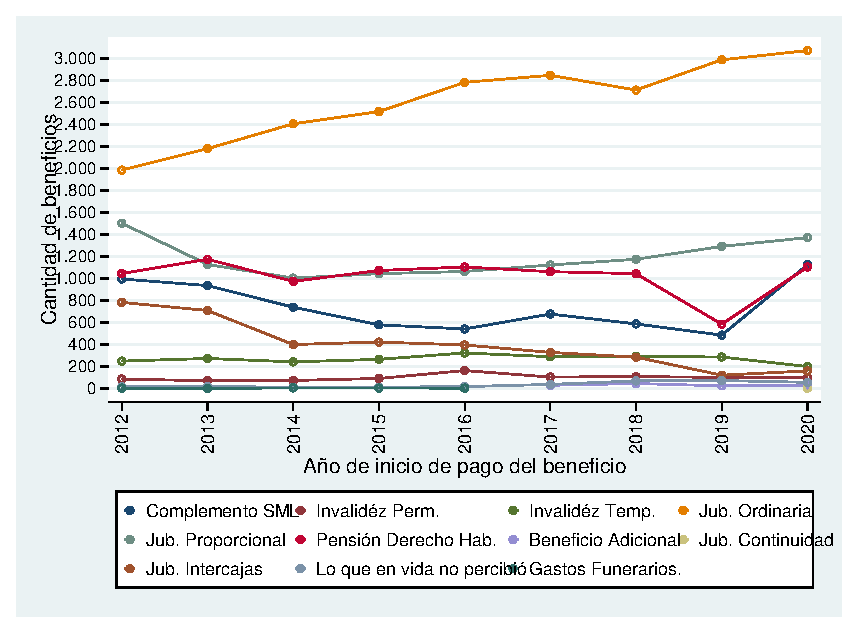
\includegraphics[scale=0.9]{RA_IPS_altas_clasif2_year.eps}
                    \item \footnotesize Fuente : Registros administrativos del IPS. 
                    \end{center}
\end{figure}

\textbf{***agregar el grafico de distribucion porcentual del total de nuebos beneficios pagados en J y P***}
\textbf{***agregar la tabla y el grafico de Evolucion del monto(nominal) promedio de los nuevos beneficios pagados en P y J***}

\subsubsection{Distribución de años de aportes}

El estudio de la cantidad de años de aportes con que se jubilan los
trabajadores y la densidad de aportes (años de aportes / años
trabajados) pone de manifiesto parte de la estructura de la movilidad
laboral, así como la entrada y salida del sistema, lo cual es sumamente
importante que sea representado adecuadamente en la construcción de un
modelo.

El Gráfico xx muestra como casi la mitad de los nuevos pagos por
Jubilaciones Ordinarias corresponden a trabajadores con 25 a 29 años de
antigüedad (xx\%), los restantes son trabajadores que se benefician con
la Jubilación Ordinaria concedida con al men os 30 años de antigüedad,
en tanto que, los nuevos pagos en Jubilaciones Proporcionales se dan en
un xx\% a trabajadores con 15 a 19 años de antigüedad. El xx\% restante
tiene 20 o más años de aportes acumulados. Por otra parte, en lo
concerniente a la Jubilación por Invalidez, no se requiere de ninguna
antigüedad, cuando se trata de accidentes de trabajo, por lo que se
observa una importante demanda en los trabajadores con pocos años de
antigüedad acumulados.

\textbf{***agregar gráfico de distribución porcentual de los nuevos beneficios pagados en jubilaciones por tipo de beneficio, según tramo de antiguedad***}

En el Gráfico xx se representan los nuevos beneficios pagados en
Jubilaciones Ordinarias (JO) en función a la edad de retiro y los años
de aportes (antigüedad), donde claramente se puede apreciar que la mayor
cantidad de personas accede al beneficio con los requisitos mínimos (60
años de edad y 25 años de aportes), y a partir de ahí le siguen las
personas que ya cuentan con uno de los requisitos (edad o antigüedad) y
acceden al beneficio una vez cumplido el segundo requisito.

\textbf{***agregar gráfico de cantidad de nuevos beneficios pagados en jubilación ordinaria por año de antigüedad, según tramos de edad***}

En los casos de Jubilaciones Ordinarias Anticipadas
(JOA)\footnote{La base de datos de Jubilaciones no distingue entre los conceptos de Jubilación Ordinaria y Jubilación Ordinaria Anticipada, la clasificación dada se ha conseguido mediante la revisión d
e las edades de retiro y los años de aporte para cada prestación.} ,
donde se requiere al menos 55 años de edad y 30 años de aportes, el
comportamiento es bastante similar cuando se los compara por edad de
retiro.

Un dato interesante es que, si bien el número es bajo, existen personas
que ya no desean o no pueden seguir aportando hasta la edad mínima
requerida (60 años) para obtener el 100\% de tasa de sustitución y se
retiran con años de aportes superiores a los 35 años (con al menos 55
años de edad).

En el caso de la Jubilación Proporcional no existe una clara tendencia
salvo que la mayor cantidad de beneficios se otorgaron a quienes
contaban con 15 años de antigüedad. Como la Ley entró en vigencia en el
año 2011, recién desde ese momento tuvieron oportunidad de acceder a un
beneficio las personas que contaban con la edad (65 años) pero no
llegaban al mínimo de 25 años de antigüedad (Ver Gráfico xx).

\textbf{agregar gráfico de cantidad de nuevos beneficios pagados en jubilación proporcional por ano de antigüedad, según tramos de edad}
